\documentclass[a4paper,12pt]{article}

\usepackage[french]{babel}
\usepackage[T1]{fontenc}
%\usepackage[utf8]{inputenc}
\usepackage{graphicx}
\usepackage{authblk}
%\usepackage{amsmath}
%\usepackage{amsfonts}
%\usepackage{amssymb}
%\usepackage{amsthm}
%\usepackage{array}
%\usepackage{enumerate}


\usepackage{hyperref}


\title{\bf Jeu de Nim : l'IA en boîte (d'allumettes)}
\author{Jean-Baptiste Caillau}
\author{Christophe Cazanave}
\author{Marc Monticelli}
\affil{Université Côte d’Azur, CNRS, LJAD, France}
\date{}

\begin{document}

\maketitle
\label{jeu-de-nim-lia-en-boite-dallumettes}

\begin{itemize}
\item
  \textbf{Niveau} : 6ème à Terminale
\item
  \textbf{Durée} : 1h30
\item
  \textbf{Objectifs} : expliquer les idées sous-jacentes à l'\emph{apprentissage par renforcement} utilisé en intelligence artificielle, illustrer le besoin de mathématiciens dans des applications désormais omniprésentes
\item
  \textbf{Pré-requis} : aucun
\item
  \textbf{Notions} : jeu, stratégie, algorithme
\item
  \textbf{Matériel} (par binôme) : 8 allumettes, $50 \times 3 = 150$ billes (ou perles à repasser\ldots) de 3 couleurs différentes, 8 boîtes d'allumettes
\end{itemize}

\section{Introduction (5 min)} \label{introduction-5-min}
\noindent On parle beaucoup des avancées spectaculaires récentes en intelligence artificielle (\href{https://www.ibm.com/ibm/history/ibm100/us/en/icons/deepblue}{DeepBlue}, \href{https://www.deepmind.com/research/highlighted-research}{AlphaGo}, \href{https://openai.com/blog/chatgpt}{chatGPT})~: comment fonctionnent ces ``machines'' qui battent désormais systématiquement les grands maîtres d'échecs, de go, rédigent des programmes informatiques... ou des dissertations~? Le but de cet atelier est d'ouvrir ladite machine (la boîte d'allumettes~!) et d'illustrer sur l'exemple du jeu de Nim un algorithme élémentaire d'intelligence artificielle qui apprend \emph{seul} itérativement (par \emph{renforcement}) la stratégie gagnante de ce jeu.

\section{Manipulation no. 1 (20-30 minutes)} \label{manipulation-no.-1-20-30-minutes}
\noindent Donner les règles du Jeu de Nim (on peut par exemple illustrer avec un extrait vidéo de \href{https://fortboyard.tv}{Fort Boyard})~:
\begin{enumerate}
  \item On dispose côte à côte 8 allumettes \footnote{Le nombre \(8\) est différent de \(1\) modulo \(4\), ce qui assure que le premier joueur a une stratégie gagnante.}.
  \item Les joueurs retirent chacun leur tour de 1 à 3 allumettes.
  \item Le joueur qui prend la dernière allumette perd la partie.
\end{enumerate}

Laisser les élèves s'approprier les règles en jouant par binômes pendant plusieurs parties. Une fois que les règles sont bien comprises, les amener à remarquer qu'ils ne peuvent jamais vous battre si vous commencez. Ils comprennent ainsi que le premier joueur a une stratégie gagnante qu'ils doivent découvrir. Cette découverte pourra être favorisée par un changement du nombre initial d'allumettes (partir de 4, 5...).  \footnote{Pour les niveaux plus avancés, on peut utiliser le vocabulaire des congruences. Pour les autres, on remarque juste qu'il y a une répétition périodique des positions gagnantes et perdantes (et des coups à jouer).}
%
Débriefer et laisser au tableau un schéma illustrant le coup gagnant à jouer en fonction du nombre d'allumettes restantes. S'assurer que tous les élèves ont bien compris la stratégie et qu'ils savent ``récupérer la main'' si le premier joueur se trompe de coup.

\begin{figure}[h!]
\centering
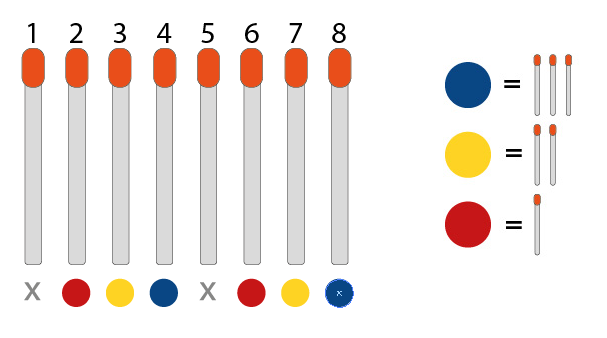
\includegraphics[scale = 0.4]{./Images/fig2-v3.png}
\caption{Schéma des coups à jouer en fonction du nombre d'allumettes restantes}
\label{fig:schemStrategie}
\end{figure}

\section{Intelligence artificielle (5-10 minutes)} \label{intelligence-artificielle-5-10-minutes}
\noindent Le but de la suite est de construire une machine qui apprend à jouer. Insister sur le fait qu'il ne s'agit pas de
programmer la solution qu'ils viennent de trouver dans un ordinateur~: ce serait alors le programmeur qui serait
intelligent et non la machine. On propose donc un algorithme d'apprentissage automatique : la machine apprend à jouer
\emph{toute seule} ; on ne lui donne que les règles du jeu et une méthode d'apprentissage pour s'améliorer partie après
partie. On peut illustrer avec l'histoire des échecs et comparer les programmes classiques (type \emph{Stockfish}) et le
programme révolutionnaire \emph{AlphaZero}. Les élèves sont intéressés aussi par les machines qui jouent seules aux jeux
vidéos.\footnote{On peut donner un rapide aperçu des différentes formes d'intelligence artificielle que l'on ne va pas
illustrer (apprentissage supervisé et apprentissage non supervisé). Introduire le vocabulaire d'apprentissage \emph{par renforcement}.}
%
La méthode d'apprentissage repose sur deux principes très naturels~: l'exploration, en testant tous les coups possibles, et le renforcement, en privilégiant les coups qui font gagner et en oubliant ceux qui font perdre.

\section{Manipulation "à la Menace" (20-30 minutes)}
\label{manipulation-uxe0-la-menace-20-30-minutes}
\noindent On suit l'idée de la machine {\sc menace} (Matchbox Educable Noughts and Crosses Engine) 
de Donald Michie \cite{Wiki, Michie} qui jouait au morpion, en l'adaptant au jeu de Nim.
%
Par groupe de 4, les élèves ajoutent sous chaque allumette du jeu une boîte remplie avec 4 billes de chacune des 3 couleurs. Les boîtes servent à faire jouer la machine. Lorsque c'est au tour de la machine, les élèves tirent au hasard dans la boîte de la position courante une bille et la posent devant la boîte. Chaque couleur correspond à un coup possible (prendre les mêmes couleurs que dans la figure~\ref{fig:schemStrategie}).

\begin{figure}[h!]
\centering
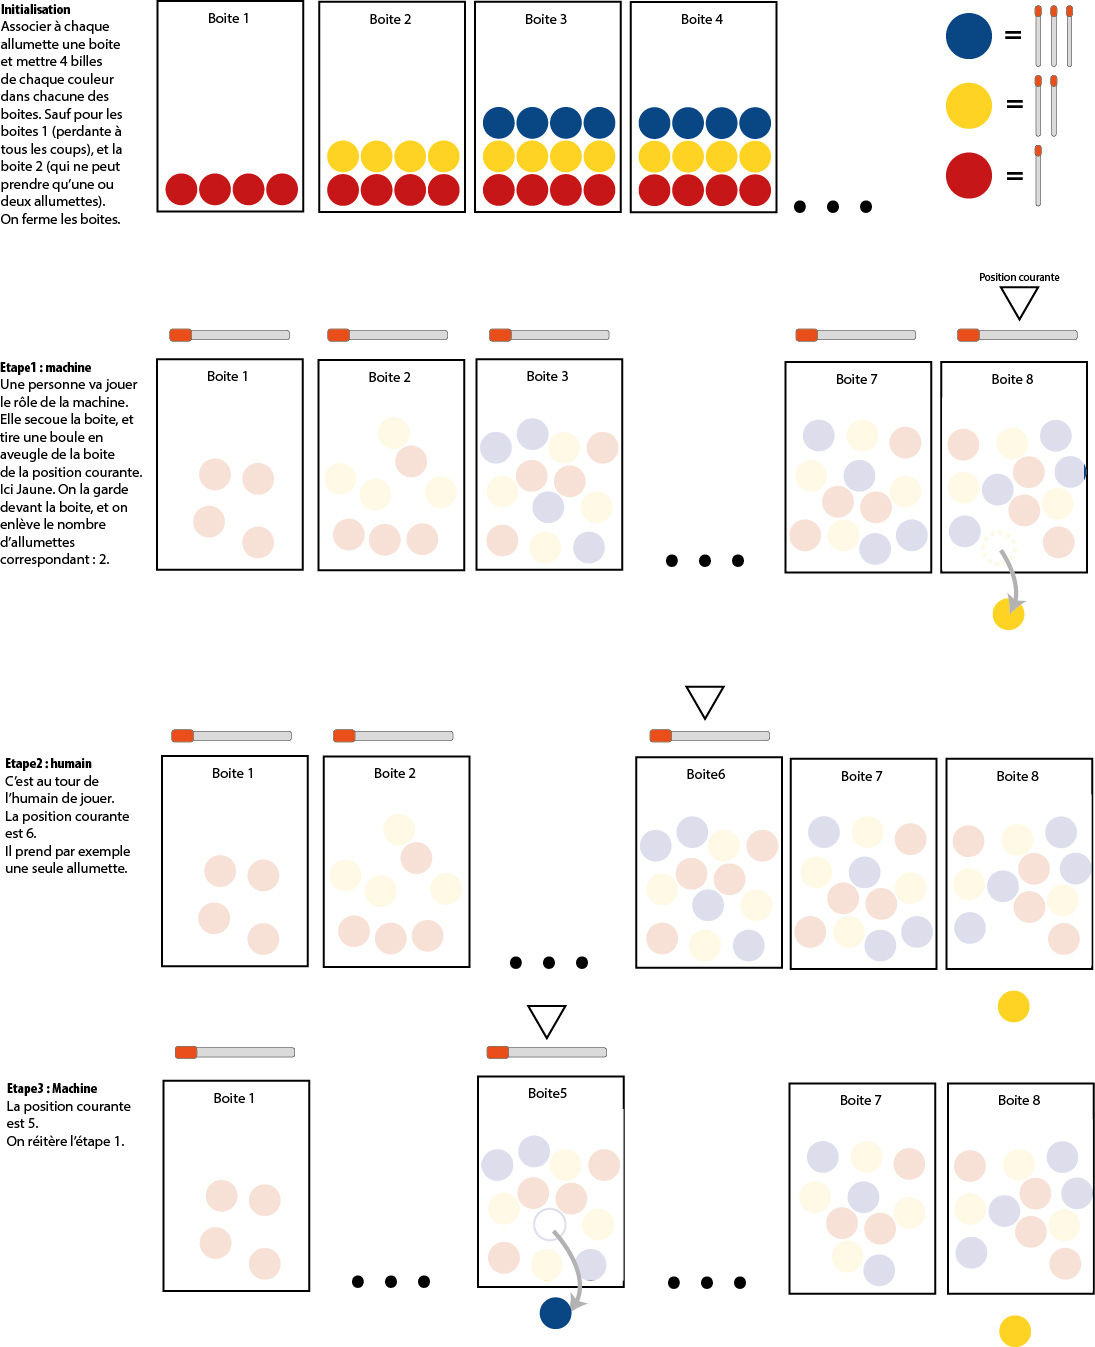
\includegraphics[scale = 0.7]{./Images/fig3-v2.jpg}
\caption{Première étape d'apprentissage de la machine.}
\label{fig:PremApprentissage}
\end{figure}

Les élèves commencent l'apprentissage de la machine en suivant le protocole des figures~\ref{fig:PremApprentissage} et \ref{fig:ProtocoleApprentissage}. 
Un binôme fait jouer la machine, l'autre binôme joue comme un expert. La machine joue en premier. À la fin de chaque partie, les élèves renforcent la machine. 
On échanger les rôles des binômes après  4 ou 5 parties.

\begin{figure}[h!]
\centering
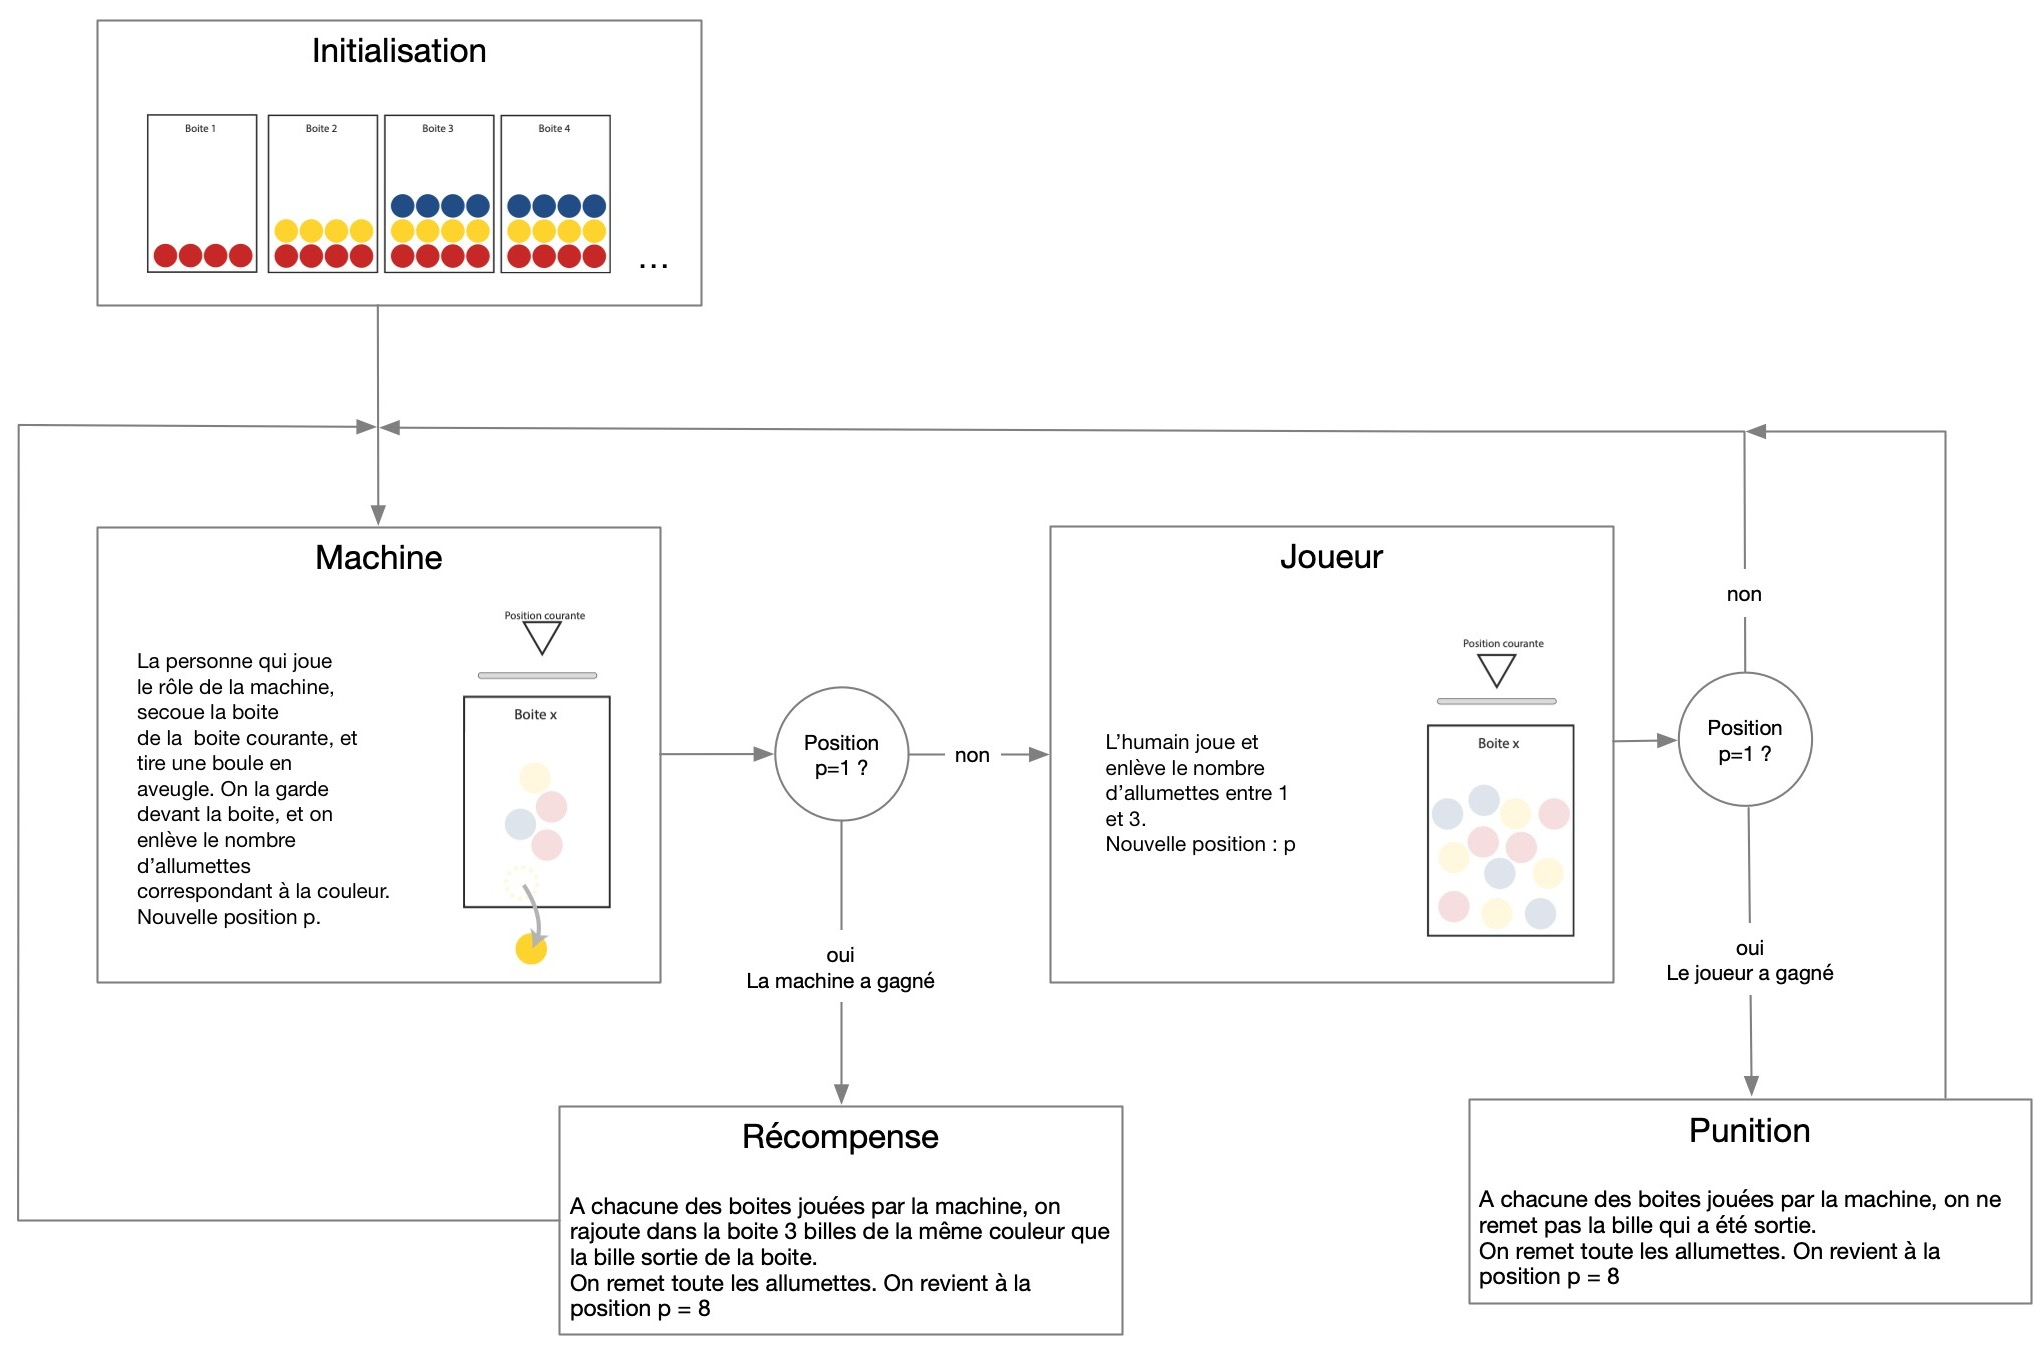
\includegraphics[scale = 0.9]{./Images/fig1-v3.jpg}
\caption{Protocole d'apprentissage de la machine.}
\label{fig:ProtocoleApprentissage}
\end{figure}

\noindent Lors de la première partie, s'assurer que les élèves ont bien compris la mise en place\footnote{Un petit détail souvent difficile à intégrer est que dans les deux premières bo\^\i tes, on ne met pas toutes les couleurs car certains coups ne sont plus possibles.} et comment faire jouer la machine\footnote{Au bout d'un moment, il peut arriver qu'une boîte ne contienne plus de billes du tout.Dans ce cas, on réinitialise la boîte avec 4 billes de chaque couleur.} et comment effectuer la phase de renforcement.
%
On constate empiriquement qu'il faut environ 100 parties pour obtenir une machine experte. Pour une fête de la science, on doit pouvoir atteindre ce nombre de parties. Pour une activité en classe, c'est trop fastidieux, on peut passer alors à une simulation numérique après avoir joué une dizaine de parties et constaté que la machine commence parfois à gagner.
%Si elle a gagné, les élèves rajoutent 4 billes de la même couleur dans la boîte en (\emph{récompense})~; si elle a perdu, les élèves retirent les billes correspondant aux coups joués par la machine.

\section{Simulation numérique} \label{simulation-numuxe9rique}
\noindent Une \href{https://u.pcloud.link/publink/show?code=XZsn7zVZrWj4xUeBzmhLp8Pxd7ismY5ezrMX}{applet
java} est disponible sur le site de la MMI\cite{MMI} à Lyon. Constater que la machine obtient le motif périodique de la stratégie gagnante (voir Fig.1). Commenter le cas des boîtes correspondant aux positions perdantes (il y restera des billes de plusieurs couleurs). Montrer et commenter les différences de rapidité de convergence selon que le second joueur est naïf, expert ou que la machine joue contre elle-même.
%
On peut conclure en insistant sur toutes les questions mathématiques liées à ce genre d'algorithme (par exemple, autour de la vitesse de convergence) et sur l'utilité de former de former des étudiants compétents en mathématiques et en informatique.

Pour aller plus loin, on pourra consulter l'article récent \cite{FrankPrivat} de la gazette,
voire se reporter à l'ouvrage de référence sur le sujet \cite{SuttonBarto}.
% 
% \subsection{Pour aller plus loin}
% \label{pour-aller-plus-loin}
% 
% L'apprentissage par renforcement se modélise bien dans le contexte du contrôle optimal discret stochastique (voir l'ouvrage de Sutton et Barto), ce qui revient à considérer un problème de la forme suivante~: maximiser l'espérance de la somme des récompenses
% 
% \[ E\left(\sum_{t=0}^{N-1} R(x_t,u_t)\right) \to \max \]
% 
% où le temps \(t=0,\dots,N-1\) est discret (\(N\) est l'horizon, fini, du jeu), et où \(R\) est la fonction qui modélise la récompense (elle peut être négative, auquel cas c'est une punition) obtenue en fonction de l'état courant du jeu, \(x_t\), et du coup joué, \(u_t\) (c'est le contrôle ou \emph{action} exercée sur le système). L'évolution de l'état du jeu est modélisé par une dynamique discrète (en général stochastique),
% 
% \[ x_{t+1} = f(x_t,u_t,e_t),\quad t \geq 0, \]
% 
% où \(x_0\) est fixé et où \(e_t\) est un processus à temps discret. Pour simplifier (!), faisons tendre \(N\) vers l'infini (partie très longue) en considérant un coût un peu renormalisé à l'aide d'un \emph{discount factor} \(\gamma \in ]0,1[\) selon
% 
% \[ E\left(\sum_{t=0}^\infty \gamma^t R(x_t,u_t)\right) \to \max. \]
% 
% Définissons la \(Q\)-fonction (c'est presque la fonction valeur du problème de maximisation)
% 
% \[ Q(x,u) := \max_{u_1,\ \dots} \left\{ E\left(\sum_{t=0}^\infty \gamma^t R(x_t,u_t)\right) \ |\ x_0 = x, u_0 = u \right\}. \]
% 
% Connaître cette fonction équivaut à savoir de jouer de façon optimale puisque, dans l'état \(x\) du jeu, il suffit de choisir son coup \(u\) parmi ceux qui maximisent la valeur \(Q(x,u)\). La programmation dynamique nous apprend que cette \(Q\)-fonction vérifie l'équation de point-fixe ci-dessous :
% 
% \[ Q(x,u) = R(x,u) + \gamma E(\max_{u'} Q(f(x,u,e_0),u')). \]
% 
% Dans le cas d'un jeu possédant un nombre fini (en général très grand) de coups et d'états possibles, il ``suffit'' donc d'apprendre une approximation suffisamment bonne de la solution de cette équation de point fixe, c'est à dire du tableau des valeurs possibles \(Q(x_i,u_j)\) indexé par les états et les coups. C'est le principe du \(Q\)-learning, qui utilise un très grand de nombre d'épisodes du jeu pour renforcer et améliorer l'approximation de ce tableau, et est à la base de nombreux algorithmes d'apprentissage. On trouvera plus d'informations et de références sur le sujet dans le numéro d'octobre 2022 de la \emph{Gazette de la SMF}.

\begin{thebibliography}{100} \label{ruxe9fuxe9rences}

\bibitem{Michie}
Michie, D. Experiments on the Mechanization of Game-Learning Part I.
  Characterization of the Model and its parameters. 
  \emph{Comput. J.} \textbf{6} (1963), 232-236.

\bibitem{Wiki}
\href{https://en.wikipedia.org/wiki/Matchbox_Educable_Noughts_and_Crosses_Engine}{Wikipedia on \emph{Matchbox Educable Noughts and Crosses Engine}}
  
\bibitem{FrankPrivat}
Franck, E.; Privat, Y. Contrôler, optimiser, décider. \emph{Gazette de la SMF} \textbf{174} (2022), 9-21.
  
\bibitem{MMI}
\href{https://mmi-lyon.fr/jouer-au-jeu-de-nim-contre-une-machine}{Jouer au de NIM contre une machine, Maison des Mathématiques et de l'informatique de Lyon}.
  
\bibitem{SuttonBarto}
\href{https://web.stanford.edu/class/psych209/Readings/SuttonBartoIPRLBook2ndEd.pdf}{Sutton,  R. S. ; Barto, A. G. Reinforcement learning : an introduction, MIT press, 2015.}
\end{thebibliography}

\end{document}
